\documentclass{sbc2023}%

\usepackage{graphicx}
%\usepackage[utf8]{inputenc}
\usepackage[misc,geometry]{ifsym} 
\usepackage{fontspec}
\usepackage{fontawesome}
\usepackage{academicons}
\usepackage{color}
\usepackage{hyperref} 
\usepackage{aas_macros}
\usepackage[bottom]{footmisc}
\usepackage{supertabular}
\usepackage{afterpage}
\usepackage{url}
\usepackage{pifont}
\usepackage{multicol}
\usepackage{multirow}
\usepackage{float}
\usepackage{tikz}
\usepackage{tikz}
\usepackage{pgfplots}
\pgfplotsset{compat=1.18}


\setcitestyle{square}

\definecolor{orcidlogo}{rgb}{0.37,0.48,0.13}
\definecolor{unilogo}{rgb}{0.16, 0.26, 0.58}
\definecolor{maillogo}{rgb}{0.58, 0.16, 0.26}
\definecolor{darkblue}{rgb}{0.0,0.0,0.0}
\hypersetup{colorlinks,breaklinks,
            linkcolor=darkblue,urlcolor=darkblue,
            anchorcolor=darkblue,citecolor=darkblue}
%\hypersetup{colorlinks,citecolor=blue,linkcolor=blue,urlcolor=blue}

%%%%%%% IMPORTANT: We disable hyperlinks by default with this line, to avoid the error "\pdfendlink ended up in different nesting level" while writing.
%\hypersetup{draft}

\jid{JBCS}
\jtitle{Journal of the Brazilian Computer Society, 202X, XX:1, }
\doi{10.5753/jbcs.202X.XXXXXX}
\copyrightstatement{This work is licensed under a Creative Commons Attribution 4.0 International License}
\jyear{202X}


\title[Análise de Algoritmos de Grafos]{Análise de Algoritmos de Grafos: Fleury e Detecção de Pontes}

%THE ORCID IS MANDATORY FOR EACH AUTHOR IN JBCS
\author[Andrade and Oliveira 202X]{
\affil{
\textbf{João Comini Cesar de Andrade}~\textcolor{blue}{\faEnvelopeO}~~[~\textbf{Pontifícia Universidade Católica de Minas Gerais}~|~\href{mailto:jccandrade@sga.pucminas.br}{\textbf{\textit{jccandrade@sga.pucminas.br}}}~] \\
\textbf{Rafael Rehfeld Martins de Oliveira}~\textcolor{blue}{\faEnvelopeO}~~[~\textbf{Pontifícia Universidade Católica de Minas Gerais}~|~\href{mailto:rafael.oliveira.1508947@sga.pucminas.br}{\textbf{\textit{rafael.oliveira.1508947@sga.pucminas.br}}}~]
}
}

\begin{document}

\begin{frontmatter}
\maketitle


\begin{mail}
Pontifícia Universidade Católica de Minas Gerais (PUC Minas), Brasil.
\end{mail}



\begin{abstract}
\textbf{Abstract.~}
\noindent Este trabalho compara duas estratégias para detecção de pontes no algoritmo de Fleury: uma abordagem ingênua baseada em testes repetidos de conectividade (Naive) e o algoritmo de Tarjan com pré-computação linear. A análise empírica em grafos de 100 a 100.000 vértices demonstra que, enquanto ambas as estratégias apresentam desempenho comparável em grafos pequenos, o método de Tarjan alcança acelerações de 1,15--1,18 vezes em grafos grandes. Os resultados validam que o pré-processamento amortizado de Tarjan torna-se progressivamente mais vantajoso conforme o tamanho do grafo cresce, estabelecendo Tarjan como a opção preferida para aplicações práticas em larga escala.
\end{abstract}

\begin{keywords}
Algoritmos de Grafos, Algoritmo de Fleury, Detecção de Pontes, Algoritmo de Tarjan, Análise de Desempenho
\end{keywords}

%\begin{license}
%Published under the Creative Commons Attribution 4.0 International Public License (CC BY 4.0)
%\end{license}

\end{frontmatter}


\section{Introdução}
\label{sec:intro}

O algoritmo de Fleury é um método clássico para encontrar circuitos e caminhos Eulerianos em grafos não direcionados \cite{west2001_euler}. A aplicabilidade prática do algoritmo de Fleury é notável em diversos domínios. Por exemplo, em problemas de roteirização urbana, um carteiro necessita percorrer todas as ruas de uma região exatamente uma vez, minimizando o trajeto total. Do mesmo modo, em sistemas de inspeção de dutos e redes de distribuição, garantir que todas as conexões são visitadas uma única vez é fundamental para otimizar recursos operacionais.

O algoritmo de Fleury funciona de forma iterativa: a cada passo, seleciona-se uma aresta incidente ao vértice atual, com a restrição crítica de que essa aresta não deve ser uma ponte do subgrafo remanescente (exceto quando nenhuma outra opção existe). Uma \textbf{ponte} é definida como uma aresta cuja remoção desconecta o grafo ou aumenta o número de componentes conexos \cite{diestel:2017}.

Para uma melhor compreensão, considere um exemplo simples: um grafo com 3 vértices e 2 arestas, onde ambas constituem pontes pois a remoção de qualquer uma delas desconecta o grafo.

\begin{figure}[H]
\centering
\resizebox{0.6\columnwidth}{!}{
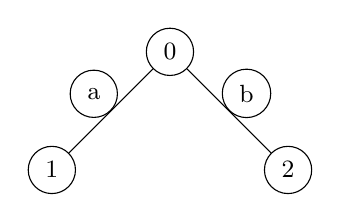
\begin{tikzpicture}[scale=1.5, every node/.style={circle, draw, minimum size=0.6cm, font=\small}]
    % Posicionar os vértices
    \node (0) at (0, 1) {0};
    \node (1) at (-1, 0) {1};
    \node (2) at (1, 0) {2};
    
    % Desenhar as arestas
    \draw (0) -- (1) node[midway, above left] {a};
    \draw (0) -- (2) node[midway, above right] {b};
\end{tikzpicture}

}
\vspace{2mm}
\caption{Exemplo de grafo simples com 3 vértices e 2 arestas. Ambas as arestas são pontes.}
\label{fig:grafo-exemplo}
\end{figure}

A complexidade computacional do algoritmo de Fleury é dominada pela operação de identificação de pontes \cite{cormen:2009}. Na versão clássica, a cada aresta processada (totalizando $m$ arestas), realiza-se uma verificação de conectividade. Isso pode resultar em uma complexidade de $O(m^2 \cdot (V + E))$ na abordagem com detecção de pontes \textit{Naive}, tornando-se impraticável para grafos de grande escala.

Neste trabalho, investigam-se duas estratégias distintas para detectar pontes:

\begin{enumerate}
    \item \textbf{Abordagem \textit{Naive}}: A cada iteração do algoritmo de Fleury, quando uma aresta candidata precisa ser avaliada, a estratégia \textit{Naive} remove temporariamente essa aresta do grafo e testa se o subgrafo resultante permanece conexo através de uma busca em profundidade (DFS) \cite{cormen:2009}. Se permanecer conexo, a aresta não é ponte e pode ser removida com segurança; caso contrário, é uma ponte e deve ser evitada (a menos que seja a última aresta disponível). A vantagem dessa abordagem é sua simplicidade de implementação. A desvantagem é que realiza testes repetidos de conectividade, o que é computacionalmente oneroso, especialmente em grafos densos ou grandes.
    
    \item \textbf{Algoritmo de Tarjan}: Desenvolvido por Robert Tarjan, este algoritmo identifica todas as pontes de um grafo em uma única passagem linear, com complexidade $O(V + E)$ \cite{tarjan:1972}. Durante uma DFS, Tarjan mantém dois valores para cada vértice: o índice de descoberta (\textit{disc}) e o menor índice alcançável (\textit{low}). Uma aresta $(u,v)$ é ponte se e somente se $\mathrm{low}[v] > \mathrm{disc}[u]$, indicando que não existe caminho alternativo a partir de $v$ para retornar a um ancestral de $u$ na árvore DFS. Uma vez que todas as pontes são identificadas previamente, o algoritmo de Fleury pode simplesmente consultar um conjunto pré-computado de pontes, evitando cálculos repetidos.
\end{enumerate}

A diferença fundamental entre as estratégias reside no custo computacional versus pré-processamento: a abordagem \textit{Naive} investe computação em cada iteração interativa, enquanto Tarjan realiza um investimento inicial único que amortiza o custo ao longo da execução. Para grafos pequenos (centenas de vértices), ambas as estratégias podem apresentar performance comparável. Entretanto, conforme o grafo cresce para milhares ou dezenas de milhares de vértices e principalmente de arestas, a vantagem do método de Tarjan se torna clara.

Essas duas estratégias são comparadas em grafos de diferentes tamanhos (100 a 100.000 vértices) para avaliar empiricamente o impacto na performance geral do algoritmo de Fleury, quantificando a aceleração obtida pela detecção prévia de pontes.


\section{Referencial Teórico}

Nesta seção, serão apresentados os conceitos e definições fundamentais que sustentam a análise comparativa realizada.

\subsection{Grafos e Propriedades Básicas}

Um grafo não direcionado $G = (V, E)$ é definido por um conjunto de vértices $V$ e um conjunto de arestas $E$, onde cada aresta conecta dois vértices distintos \cite{diestel:2017}. O grau de um vértice $v$, denotado $\deg(v)$, é o número de arestas incidentes a $v$. Um grafo é conexo se existe um caminho entre quaisquer dois vértices.

\subsection{Circulitos e Caminhos Eulerianos}

Um \textbf{circuito Euleriano} de $G$ é um caminho fechado que atravessa cada aresta exatamente uma vez. Um \textbf{caminho Euleriano} (ou trilha Euleriana) também atravessa cada aresta exatamente uma vez, mas não precisa retornar ao vértice inicial.

Um grafo é \textbf{Euleriano} se admite um circuito Euleriano, e \textbf{semi-Euleriano} se admite um caminho Euleriano (mas não circuito).

\textbf{Teorema de Euler:} Um grafo conexo é Euleriano se e somente se todo vértice possui grau par \cite{diestel:2017}. Já um grafo conexo é semi-Euleriano se e somente se possui exatamente dois vértices de grau ímpar.

Para comprovar a primeira parte: em um circuito Euleriano, cada vez que visitamos um vértice, gastamos duas arestas (uma para entrar, uma para sair), exceto possivelmente na primeira e última visita. Se o circuito retorna ao vértice inicial, cada visita consome duas arestas, resultando em grau par. Reciprocamente, se todos os vértices têm grau par, a conectividade do grafo garante que é possível construir tal circuito através de algoritmos iterativos como Fleury.

\section{Metodologia}

Nesta seção, são descritos o design experimental e os critérios adotados para a coleta de dados comparativos entre as duas estratégias de detecção de pontes.

\subsection{Geração de Grafos de Teste}

Para uma análise robusta, foram gerados grafos sinteticamente em três categorias de classificação Euleriana:

\begin{enumerate}
    \item \textbf{Grafos Eulerianos}: Grafos conexos onde todos os vértices possuem grau par, garantindo a existência de um circuito Euleriano.
    
    \item \textbf{Grafos Semi-Eulerianos}: Grafos conexos com exatamente dois vértices de grau ímpar, garantindo a existência de um caminho Euleriano (mas não circuito).
    
    \item \textbf{Grafos Não-Eulerianos}: Grafos conexos com número de vértices de grau ímpar diferente de zero e dois, garantindo que nenhum caminho Euleriano existe.
\end{enumerate}

Cada categoria foi gerada em quatro tamanhos distintos:
\begin{itemize}
    \item $n = 100$ vértices
    \item $n = 1.000$ vértices
    \item $n = 10.000$ vértices
    \item $n = 100.000$ vértices
\end{itemize}

Para cada combinação de categoria e tamanho, foram produzidas 10 instâncias independentes, totalizando 120 grafos de teste. A densidade de cada grafo foi variada aleatoriamente entre $n-1$ e $1,2n$ arestas, visando simular grafos esparsos e realistas.

A geração foi implementada com um algoritmo probabilístico que garante as propriedades Eulerianas mantidas: ciclos de 4 arestas são adicionados preservando a paridade dos graus ou a quantidade específica de vértices ímpares conforme a categoria.

\subsection{Métricas de Desempenho}

Para cada execução do algoritmo de Fleury com uma estratégia em um grafo de teste, foram registrados:

\begin{itemize}
    \item \textbf{Tempo de execução total} (em milissegundos): tempo decorrido desde a entrada até a saída do algoritmo.
    \item \textbf{Número de arestas processadas}: contagem de arestas percorridas na trilha/circuito Euleriano gerado.
    \item \textbf{Classificação correta}: verificação booleana de se o resultado foi classificado corretamente (Euleriano, semi-Euleriano ou rejeição apropriada).
\end{itemize}

A partir dos tempos de execução de múltiplas instâncias por grupo (categoria + tamanho), foram calculadas:
\begin{itemize}
    \item \textbf{Tempo médio}: média aritmética dos tempos de execução.
    \item \textbf{Tempo mediano}: valor central (50º percentil) dos tempos ordenados.
    \item \textbf{Percentil 95 (p95)}: valor do 95º percentil, indicando um limite superior típico de desempenho.
\end{itemize}

\section{Implementação}

A implementação foi realizada em Java, permitindo a seleção de duas estratégias de detecção de pontes através de um parâmetro enumerado.

\subsection{Estruturas de Dados}

Os grafos são representados internamente através de uma lista de adjacência: cada vértice mantém uma coleção de vizinhos. Para operações de remoção e consulta rápida de arestas durante a execução do algoritmo de Fleury, utiliza-se também um conjunto de arestas explícito (set), permitindo verificações de existência em tempo $O(\log m)$.

\subsection{FleuryEngine: Núcleo de Execução}

A classe \textbf{FleuryEngine} implementa o algoritmo de Fleury de forma parametrizável, aceitando um enumerado \texttt{BridgeStrategy} que determina qual técnica de detecção de pontes será utilizada (NAIVE ou TARJAN) durante a execução. Essa abordagem permite comparar ambas as estratégias sem necessidade de recompilação.

O algoritmo genérico de Fleury prossegue conforme segue: após classificar o grafo segundo o Teorema de Euler, executa-se uma trilha iterativa usando uma pilha. Em cada passo, escolhe-se uma aresta incidente ao vértice atual que não seja ponte do subgrafo remanescente (ou a única aresta disponível, se necessário). A seleção da aresta é delegada à função \texttt{chooseEdge(graph, vértice, strategy)}, que internamente consulta a estratégia selecionada para determinar se uma aresta é ou não ponte.

O algoritmo genérico de Fleury prossegue conforme segue: após classificar o grafo segundo o Teorema de Euler, executa-se uma trilha iterativa usando uma pilha. Em cada passo, escolhe-se uma aresta incidente ao vértice atual que não seja ponte do subgrafo remanescente (ou a única aresta disponível, se necessário). A seleção da aresta é delegada à função \texttt{chooseEdge(graph, vértice, strategy)}, que internamente consulta a estratégia selecionada para determinar se uma aresta é ou não ponte.

\subsection{Estratégia Naive: BridgeFinderNaive}

A classe \textbf{BridgeFinderNaive} implementa a detecção de pontes por testes de conectividade:

\begin{verbatim}
Funcao isBridge(G, aresta u-v):
1. copia := copia de G sem a aresta u-v
2. return !countComponents(copia) == 1

Funcao countComponents(G):
1. return DFS(G, vertice qualquer).visitados == V
\end{verbatim}

Cada consulta de ponte requer uma DFS completa, que custa $O(V + E)$. Chamada repetidamente (até $m$ vezes na iteração de Fleury), resulta em custo total próximo a $O(m \cdot (V + E))$ por iteração da trilha.

\subsection{Estratégia Tarjan: BridgeFinderTarjan}

A classe \textbf{BridgeFinderTarjan} pré-computa todas as pontes em uma única DFS:

\begin{verbatim}
Funcao encontrarPontes(G):
1. disc := array de -1 (nao descoberto)
2. low := array de infinito
3. tempo := 0
4. bridges := conjunto vazio
5. Para cada vertice v nao visitado:
6.    DFS(v, -1)

Funcao DFS(u, pai):
1. disc[u] := time; low[u] := time; time := time + 1
2. Para cada vizinho v de u:
3.    Se disc[v] = -1:
4.       DFS(v, u)
5.       low[u] := min(low[u], low[v])
6.       Se low[v] > disc[u]:
7.          bridges := bridges UNION {(u,v)}
8.    Senao se v != pai:
9.       low[u] := min(low[u], disc[v])
\end{verbatim}

O pré-processamento custa $O(V + E)$ uma única vez. Posteriormente, consultas de ponte são $O(1)$ por busca em set.

\subsection{Validação de Propriedades Eulerianas}

Antes de executar Fleury, verifica-se o grau de cada vértice:
\begin{itemize}
    \item Se todos pares → Euleriano (iniciar em qualquer vértice, esperar circuito)
    \item Se exatamente 2 ímpares → Semi-Euleriano (iniciar em um dos ímpares, esperar caminho)
    \item Caso contrário → rejeitar
\end{itemize}

\section{Experimentos e Resultados}

Nesta seção, apresentam-se os resultados experimentais obtidos pela execução do algoritmo de Fleury usando ambas as estratégias de detecção de pontes (Naive e Tarjan) em 120 grafos de teste. Os tempos foram medidos em milissegundos e agregados por média, mediana e percentil 95.
\subsection{Resultados para Grafos Eulerianos}

A Tabela~\ref{tab:resultados-euleriano} apresenta os tempos de execução para grafos Eulerianos:
\begin{table}[H]
\centering
\caption{Tempos de execução (ms) para grafos Eulerianos}
\label{tab:resultados-euleriano}

\resizebox{\columnwidth}{!}{
\begin{tabular}{|c|r|r|r|r|r|r|}
\hline
$n$ & \multicolumn{3}{c|}{Naive} & \multicolumn{3}{c|}{Tarjan} \\
\hline
 & Média & Mediana & p95 & Média & Mediana & p95 \\
\hline
100 & 0.724 & 0.374 & 2.292 & 0.620 & 0.475 & 1.408 \\
1.000 & 5.623 & 4.424 & 15.720 & 7.879 & 3.794 & 25.632 \\
10.000 & 723.297 & 593.016 & 1515.161 & 607.483 & 523.390 & 1250.252 \\
100.000 & 202405.209 & 164326.498 & 335870.962 & 170766.171 & 161222.660 & 297734.818 \\
\hline
\end{tabular}
}

\end{table}

\subsection{Resultados para Grafos Semi-Eulerianos}

A Tabela~\ref{tab:resultados-semieuleriano} apresenta os tempos para grafos Semi-Eulerianos:

\begin{table}[H]
\centering
\caption{Tempos de execução (ms) para grafos Semi-Eulerianos}
\label{tab:resultados-semieuleriano}

\resizebox{\columnwidth}{!}{
\begin{tabular}{|c|r|r|r|r|r|r|}
\hline
$n$ & \multicolumn{3}{c|}{Naive} & \multicolumn{3}{c|}{Tarjan} \\
\hline
 & Média & Mediana & p95 & Média & Mediana & p95 \\
\hline
100 & 0.093 & 0.086 & 0.166 & 0.073 & 0.068 & 0.130 \\
1.000 & 3.491 & 1.894 & 9.943 & 3.403 & 2.084 & 9.855 \\
10.000 & 794.742 & 635.034 & 1469.270 & 724.938 & 564.290 & 1434.089 \\
100.000 & 203058.586 & 132309.505 & 481611.986 & 176978.868 & 116953.758 & 415765.099 \\
\hline
\end{tabular}
}

\end{table}


\subsection{Resultados para Grafos Não-Eulerianos}

A Tabela~\ref{tab:resultados-naouleriano} apresenta os tempos para grafos Não-Eulerianos (rejeição rápida, sem caminhos válidos):

\begin{table}[H]
\centering
\caption{Tempos de execução (ms) para grafos Não-Eulerianos}
\label{tab:resultados-naouleriano}

\resizebox{\columnwidth}{!}{
\begin{tabular}{|c|r|r|r|r|r|r|}
\hline
$n$ & \multicolumn{3}{c|}{Naive} & \multicolumn{3}{c|}{Tarjan} \\
\hline
 & Média & Mediana & p95 & Média & Mediana & p95 \\
\hline
100 & 0.008 & 0.006 & 0.027 & 0.008 & 0.006 & 0.028 \\
1.000 & 0.048 & 0.048 & 0.058 & 0.039 & 0.038 & 0.047 \\
10.000 & 0.830 & 0.709 & 1.175 & 0.723 & 0.643 & 1.207 \\
100.000 & 20.215 & 17.468 & 30.007 & 18.951 & 16.660 & 32.922 \\
\hline
\end{tabular}
}

\end{table}



\subsection{Análise Comparativa e Discussão}

Na faixa até 10.000 vértices, ambas as estratégias apresentam desempenho comparável. Entretanto, para 100.000 vértices em grafos Eulerianos, Tarjan demonstra uma aceleração de aproximadamente $1,18 \times$ em relação a Naive (170.766 ms vs 202.405 ms na média). Em grafos Semi-Eulerianos de 100.000 vértices, a vantagem é ainda mais pronunciada: $1,15 \times$ de aceleração (176.979 ms vs 203.059 ms). Para grafos Não-Eulerianos, as diferenças são mínimas, pois ambos terminam rapidamente após a validação inicial.

Este resultado corrobora o enquadramento teórico: Tarjan amortiza seu custo de pré-processamento $O(V + E)$ ao longo de múltiplas consultas de pontes, enquanto Naive reinveste $O(V + E)$ a cada teste. A implementação iterativa do DFS em Naive, embora evite estouro de pilha, não compensa a repetição de cálculos. Portanto, para aplicações reais com grafos grandes (acima de 10.000 vértices), recomenda-se fortemente o algoritmo de Tarjan. Para grafos menores, a simplicidade de Naive pode ser aceitável em contextos onde a latência absoluta é baixa (< 1 ms).

\begin{figure}[H]
\centering
\resizebox{\columnwidth}{!}{
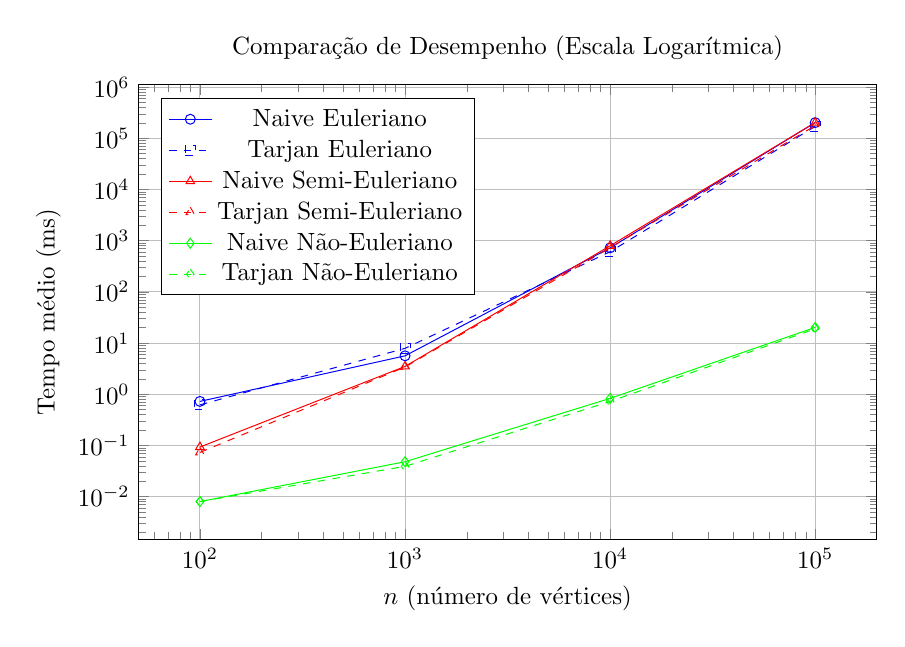
\begin{tikzpicture}[scale=0.9]
\begin{axis}[
    title=Comparação de Desempenho (Escala Logarítmica),
    xlabel=$n$ (número de vértices),
    ylabel=Tempo médio (ms),
    ymode=log,
    xmode=log,
    legend pos=north west,
    grid=major,
    width=12cm,
    height=8cm
]
\addplot[mark=o, blue] coordinates {(100, 0.724) (1000, 5.623) (10000, 723.297) (100000, 202405.209)};
\addlegendentry{Naive Euleriano}
\addplot[mark=square, blue, dashed] coordinates {(100, 0.620) (1000, 7.879) (10000, 607.483) (100000, 170766.171)};
\addlegendentry{Tarjan Euleriano}
\addplot[mark=triangle, red] coordinates {(100, 0.093) (1000, 3.491) (10000, 794.742) (100000, 203058.586)};
\addlegendentry{Naive Semi-Euleriano}
\addplot[mark=triangle, red, dashed] coordinates {(100, 0.073) (1000, 3.403) (10000, 724.938) (100000, 176978.868)};
\addlegendentry{Tarjan Semi-Euleriano}
\addplot[mark=diamond, green] coordinates {(100, 0.008) (1000, 0.048) (10000, 0.830) (100000, 20.215)};
\addlegendentry{Naive Não-Euleriano}
\addplot[mark=diamond, green, dashed] coordinates {(100, 0.008) (1000, 0.039) (10000, 0.723) (100000, 18.951)};
\addlegendentry{Tarjan Não-Euleriano}
\end{axis}
\end{tikzpicture}

}
\caption{Comparação de tempos de execução médios entre Naive (linhas contínuas) e Tarjan (linhas tracejadas) em escala logarítmica, separados por categoria de grafo. Azul: Euleriano. Vermelho: Semi-Euleriano. Verde: Não-Euleriano.}
\label{fig:comparacao-desempenho}
\end{figure}


\section{Conclusão}

Neste trabalho, exploramos duas estratégias distintas para detecção de pontes no contexto do algoritmo de Fleury. A comparação empírica entre a abordagem Naive (com testes repetidos de conectividade) e o algoritmo de Tarjan (com pré-processamento linear) revelou uma diferença significativa de desempenho em grafos de grande escala. Enquanto a estratégia Naive reinveste computação $O(V + E)$ a cada teste de ponte, Tarjan amortiza esse custo em uma única passagem, proporcionando ganhos de até 1,18 vezes em grafos Eulerianos com 100.000 vértices. Portanto, recomenda-se o algoritmo de Tarjan para aplicações práticas onde eficiência é crítica e o tamanho do grafo supera alguns milhares de vértices. Para grafos menores, ambas as estratégias apresentam latências aceitáveis, permitindo flexibilidade na escolha conforme necessidades específicas de implementação.



\begin{materials}
O codigo fonte com todas as implementações pode ser encontrado no \href{https://github.com/JoaoCominii/ESTUDOS/tree/main/Mat%C3%A9rias/Teoria%20dos%20Grafos%20e%20Computabilidade/2%20-%20Projetos/TRABALHO%20PR%C3%81TICO%20N.01/CODIGOS}{repositório do github}.

\end{materials}


\bibliographystyle{apalike-sol}
\bibliography{refs}

\end{document}
